%%\textbf{}%%%%%%%%%%%%%%%%%%%%%%%%%%%%%%%%%%%%%%%%%%%%%%%%%%%%%%%%%%%%%%%%%%%%%%%%%%%%%%
%2345678901234567890123456789012345678901234567890123456789012345678901234567890
%        1         2         3         4         5         6         7         8
% THESIS CHAPTER


\chapter{C++ Code Scheme}
\label{chap:AppendixCode}
\ifpdf
\graphicspath{{Appendix/Figures/PNG/}{Appendix/Figures/PDF/}{Appendix/Figures/}}
\else
\graphicspath{{Appendix/Figures/EPS/}{Appendix/Figures/}}
\fi

Some effort has been spent to implement a flexible and modular C++ code architecture. The main focus is directed to facilitate the use of the TPIK approach. With this scheme, adding and removing tasks from the code is easy and straightforward. Furthermore, even if ROS is used as interface, other communication methods (for different simulators, or even for real robots) can be used easily, changing a little part of the code. This is due to the fact that all the ROS parts (the \textit{interfaces}) are implemented in different files from the ones of the main blocks.\\
Only a rough idea about the code scheme is given here, without too much details. Further explanations can be found in the \href{https://github.com/torydebra/AUV-Coop-Assembly}{github page} and in the \href{https://torydebra.github.io/AUV-Coop-Assembly/}{code documentation}.

\section{Tools}
The Control Architecture is implemented in C++ language, using various libraries. In this section, the most relevant libraries and tools used for the software are described. Please note that a particular section (section \ref{sec:simulators}) is dedicated to the choice of the simulator, and another for tools used by vision (section \ref{sec:visionTools}).

\begin{itemize}
	\item \href{http://www.ros.org/}{\textbf{ROS}} (Robot Operating System), the well-known robotic middleware. It is used to communicate with the simulator, so to send commands to robots and receive information by the on-going simulations (e.g. robots states, information from sensors, streaming images from cameras).
	
	\item \href{http://eigen.tuxfamily.org/index.php?title=Main_Page}{\textbf{Eigen}} [\cite{eigen}], a C++ library for linear algebra. It is very useful to deal with matrices computations and management in any C++ software.
	
	\item \textbf{CMAT}, another C++ library, implemented at \href{http://www.graal.dibris.unige.it/}{GRAAL}. It implements the core functions for the TPIK method, detailed in \cite{IntroMaris1}.
	
	\item \href{http://www.orocos.org/kdl}{\textbf{Orocos KDL}}, a package to deal with kinematic and dynamic chains. Here it is used to compute the Jacobian of the robots, given the configurations.
\end{itemize}

\section{The Single Robot Code Scheme}
\begin{figure}[H]
	\begin{center}
		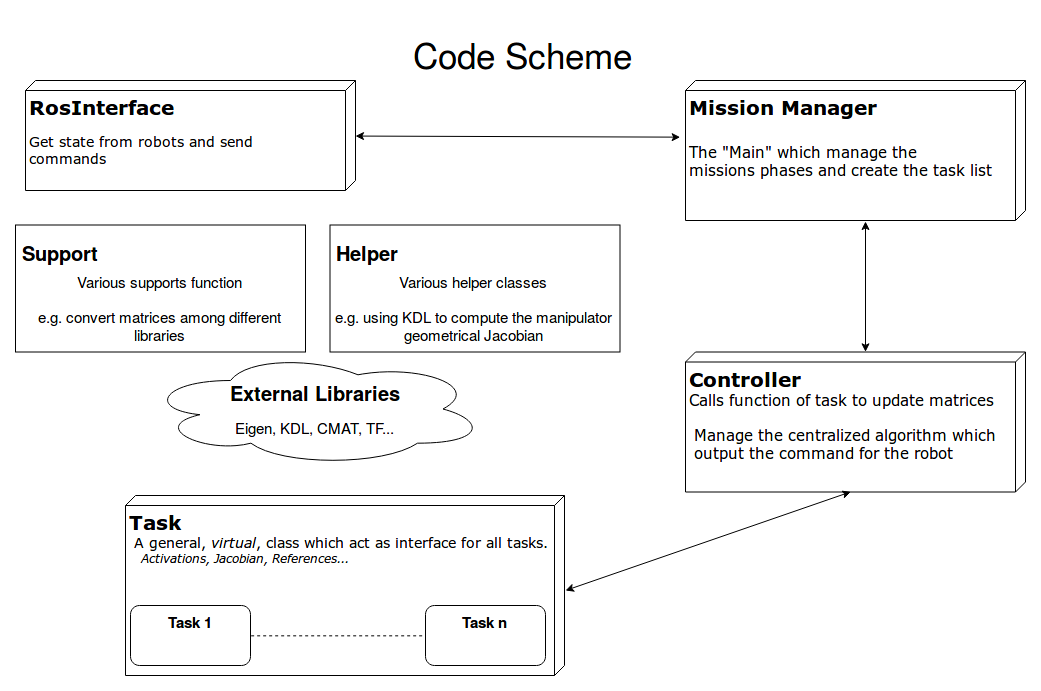
\includegraphics[width=1\columnwidth]{CodeScheme_single.png}
		\caption[C++ Code Scheme for the single robot]{The C++ code scheme that show the relationship between the main blocks of the single robot. Parallelepipeds represent the principal blocks, while rectangles contain useful functions used by them. Arrows indicate the communication between the main blocks.}
		\label{fig:codeSchemeSingle}
	\end{center}
\end{figure}

Here is presented the scheme for the two carrying robots. The two robots share the same code, and they are differentiated (when necessary) thanks to their names (\textit{g500\_A} and \textit{g500\_B}).

\begin{itemize}
	\item \textbf{RosInterface}\quad This class is used to communicate with the simulator, e.g. sending commands to the robot, receiving state and sensor information, and so on. It is obviously ROS-dependent, and it should be replaced if another middleware is used.
	
	\item \textbf{Mission Manager}\quad This block is the \enquote{main}. It initializes all useful classes, it creates the tasks list, and it manages the whole mission.
	
	\item \textbf{Controller}\quad This class is the core of the control; in practice it is the kinematic layer. It generates commands for the vehicle according to the prioritized list of tasks. It is where the iCAT algorithm (\ref{sec:tpik}) is used.
	
	\item \textbf{Task}\quad This is an \textit{abstract} class. It acts as a base class, and all the specific \textit{concrete} classes of tasks derive from this one. In this way, the controller and the mission manager simply handle a vector of pointer to Task. The Mission Manager creates a concrete class for each task and then it fills a vector. This vector is the prioritized list of the TPIK method. The controller can iterate this vector and can call the abstact methods of Task without worrying of which real concrete task is actually inside the list.
	
	\item \textbf{Support}\quad It is a group of various \textit{namespaces}, used for conversions, to print to file, and to use some mathematical formulas.
	
	\item \textbf{Helper}\quad It contains a group of classes and headers used to help the control scheme (e.g. to compute the Jacobian with KDL) and to log results.
\end{itemize}


\section{The Whole Code Scheme}
\begin{figure}[H]
	\begin{center}
		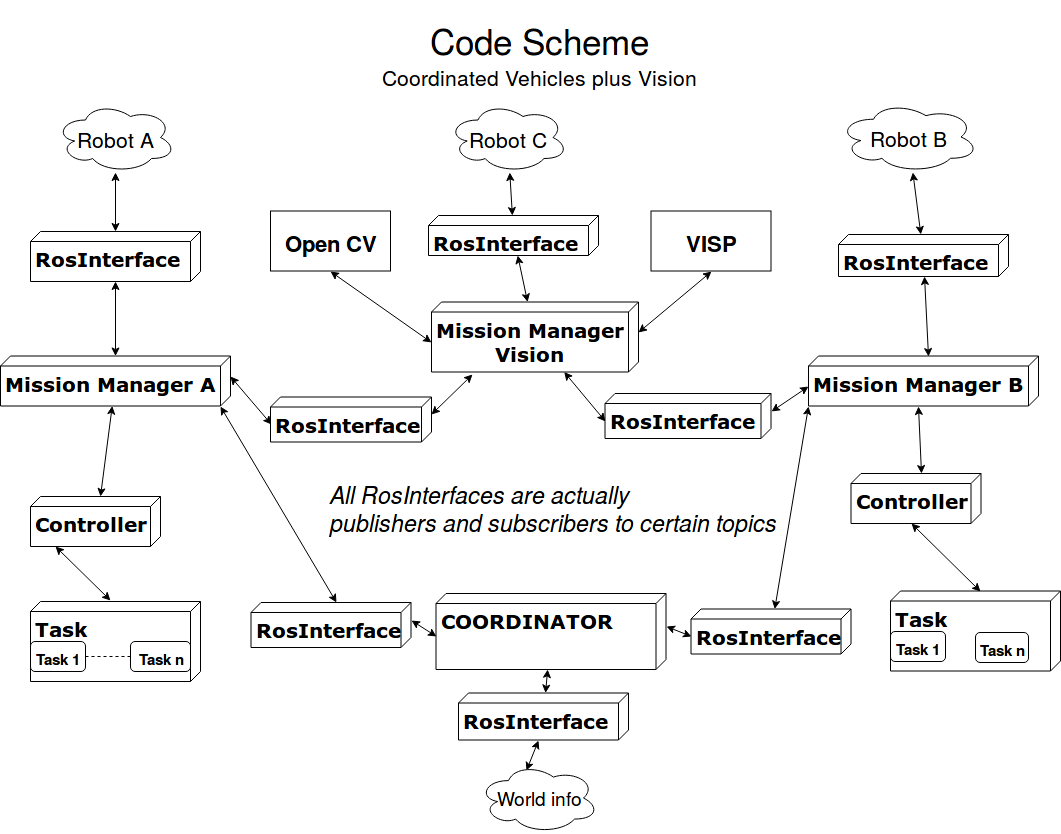
\includegraphics[width=1\columnwidth]{CodeScheme.png}
		\caption[C++ Code Scheme for the whole architecture]{The C++ code scheme that show the relationship between the main blocks of the three robots. On the left and on the right side there is a zoomed out view of the fig. \ref{fig:codeSchemeSingle}, for the two carrying robots. In the centre, there are the schemes for the Vision Robot (where also main tools for it are visible) and for the Coordinator.}
		\label{fig:codeSchemeWhole}
	\end{center}
\end{figure}
	
The two robots must communicate between them and with the vision robot. Like explained before, ROS is used to communicate with the simulator, but it is also used to make different nodes (e.g. Coordinator and Robots) to communicate.\\
Please note that the Coordinator is not a physical object: can be put as a routine on one robot. This would help communication issues, because only information exchange between the Coordinator and the other robot will pass through the water.\\
The scheme for the Vision Robot is simplify because it is driven as a ROV: so it is not autonomous and no TPIK is implemented for it. Anyway, it can be turned easily into an autonomous robot, with or without TPIK (that it is not really necessary for this robot).\\
The Coordinator is a node in charge of dealing with the coordination method explained in section \ref{sec:coopScheme}. It also needs information from the world (i.e. the simulation) to compute the cooperative velocity.
